\documentclass[a4paper,12pt]{article}

% Настройка русского языка и шрифтов для XeLaTeX
\usepackage{polyglossia} 
\setmainlanguage{russian}
\setotherlanguage{english}

\usepackage{fontspec}
\setmainfont{Times New Roman}
\setmonofont{Courier New}

\newfontfamily{\cyrillicfonttt}{Courier New} % <-- ИЛИ ТАКУЮ СТРОКУ
\usepackage{geometry}
\usepackage{setspace}
\usepackage{amsmath}
\usepackage{graphicx} 
\usepackage{listings}
\usepackage{xcolor}
\usepackage{fancybox}

% Настройка точных полей страницы
\geometry{top=20mm, bottom=20mm, left=25mm, right=15mm}

% Стиль для кода Python
\lstset{
    language=Python,
    basicstyle=\ttfamily\scriptsize,
    keywordstyle=\color{blue},
    stringstyle=\color{red},
    commentstyle=\color{green!60!black},
    numbers=left,
    numberstyle=\tiny\color{gray},
    stepnumber=1,
    numbersep=5pt,
    backgroundcolor=\color{gray!5},
    showstringspaces=false,
    breaklines=true,
    frame=single,
    rulecolor=\color{black!30}
} 

\begin{document}

% --- Горизонтальный блок: Логотип слева, текст справа ---
\noindent
\begin{minipage}[c]{0.22\textwidth}
    \centering
    % Подгоняем ширину картинки под выделенную область минипейджа
    
\includegraphics[width=\textwidth]{../bmstu_logo.jpg} 
\end{minipage}%
\hfill
\begin{minipage}[c]{0.75\textwidth}
    \centering
    \setstretch{0.95}
    {\small\bfseries Министерство науки и высшего образования Российской Федерации} \\[2pt]
    {\small\bfseries Федеральное государственное автономное образовательное учреждение} \\[2pt]
    {\small\bfseries высшего образования} \\[2pt]
    {\small\bfseries «Московский государственный технический университет} \\[2pt]
    {\small\bfseries имени Н.Э. Баумана} \\[2pt]
    {\small\bfseries (национальный исследовательский университет)»} \\[2pt]
    {\small\bfseries (МГТУ им. Н.Э. Баумана)}
\end{minipage}

\vspace{12pt}
% Двойная декоративная линия под шапкой (на всю ширину текстового поля)
\hrule height 1pt
\vspace{2pt}
\hrule height 2pt

\vspace{10mm}

% --- ФАКУЛЬТЕТ И КАФЕДРА ---
\noindent
\setstretch{1.2}
\textbf{ФАКУЛЬТЕТ} \underline{\makebox[138mm][l]{\hspace{15mm}\textbf{ИНФОРМАТИКА И СИСТЕМЫ УПРАВЛЕНИЯ}}} \\[10pt]
\textbf{КАФЕДРА} \underline{\makebox[143mm][l]{\hspace{12mm}\textbf{СИСТЕМЫ ОБРАБОТКИ ИНФОРМАЦИИ И УПРАВЛЕНИЯ}}}

\vspace{25mm}

% --- Название работы и дисциплина ---
\begin{center}
    \setstretch{1.3}
    {\Large Отчет по лабораторной работе № 1} \\[12pt]
    {\Large\bfseries «Разведочный анализ данных.} \\[4pt]
    {\Large\bfseries Исследование и визуализация данных»} \\[20mm]
    {\large по дисциплине «Технологии машинного обучения»}
\end{center}

\vspace{35mm}

% --- Блок подписей студента и преподавателя ---
\noindent
\setstretch{1.1}
\begin{tabular}{@{}llcc}
    \large Студент & \underline{\makebox[28mm][c]{\textbf{ИУ5-64Б}}} & \underline{\makebox[55mm]{}} & \underline{\makebox[50mm][c]{\textbf{Н.А. Чернев}}} \\[2pt]
    & \multicolumn{1}{c}{\scriptsize (Группа)} & \scriptsize (Подпись, дата) & \scriptsize (И.О. Фамилия) \\[20pt]
    \large Преподаватель & & \underline{\makebox[55mm]{}} & \underline{\makebox[50mm][c]{\textbf{Ю.Е. Гапанюк}}} \\[2pt]
    & & \scriptsize (Подпись, дата) & \scriptsize (И.О. Фамилия)
\end{tabular}

\vfill

% --- Год внизу ---
\begin{center}
    \large 2026 г.
\end{center}

\newpage

\pagestyle{plain}

\section*{Цель работы}
Изучение различных методов визуализации данных и проведение разведочного анализа.

\section*{Описание задания}
\begin{enumerate}
    \item Выбрать датасет без пропусков из scikit-learn.
    \item Исследовать основные характеристики: размер, типы признаков.
    \item Провести визуальный анализ через гистограммы, scatter plots, box plots.
    \item Вычислить корреляционную матрицу и интерпретировать зависимости.
\end{enumerate}

\section*{Выбранный датасет}
\textbf{Wine dataset} из scikit-learn. Датасет содержит результаты химического анализа вин трех производителей (178 образцов, 13 числовых признаков).

\subsection*{Загрузка данных и импорт библиотек}
\begin{lstlisting}
import numpy as np
import pandas as pd
import matplotlib.pyplot as plt
import seaborn as sns
from sklearn.datasets import load_wine

# Загрузка датасета
wine = load_wine()
df = pd.DataFrame(wine.data, columns=wine.feature_names)
df['target'] = wine.target
df['target_name'] = df['target'].map({0: 'class_0', 1: 'class_1', 2: 'class_2'})

# Информация о датасете
print(f"Shape: {df.shape}")  # (178, 14)
print(f"Missing values: {df.isnull().sum().sum()}")  # 0
\end{lstlisting}

\section*{Основные характеристики датасета}

\begin{itemize}
    \item \textbf{Размер:} 178 образцов, 13 признаков
    \item \textbf{Классы:} 3 класса вин (сбалансированы)
    \item \textbf{Пропуски:} отсутствуют
    \item \textbf{Признаки:} alcohol, malic\_acid, ash, flavanoids, color\_intensity, proline и др.
\end{itemize}

\subsection*{Описательные статистики}
\begin{lstlisting}
# Базовая статистика
print(df.describe())

# Проверка типов и пропусков
print(df.info())
print("Соотношение классов:", df['target'].value_counts().to_dict())
\end{lstlisting}

\section*{Визуальное исследование}

\subsection*{Распределение признаков по классам}
\begin{lstlisting}
# Гистограммы для каждого признака
fig, axes = plt.subplots(4, 4, figsize=(18, 14))
axes = axes.flatten()

colors = ['#FF6B6B', '#4ECDC4', '#45B7D1']
for i, col in enumerate(wine.feature_names):
    ax = axes[i]
    for cls in sorted(df['target'].unique()):
        data = df[df['target'] == cls][col]
        ax.hist(data, alpha=0.6, label=f'Class {cls}', color=colors[cls])
    ax.set_title(col, fontweight='bold')
    ax.set_xlabel('Значение')
    ax.set_ylabel('Частота')
    ax.legend()

plt.tight_layout()
plt.savefig('histograms.png', dpi=150, bbox_inches='tight')
plt.show()
\end{lstlisting}

\begin{figure}[h!]
    \centering
    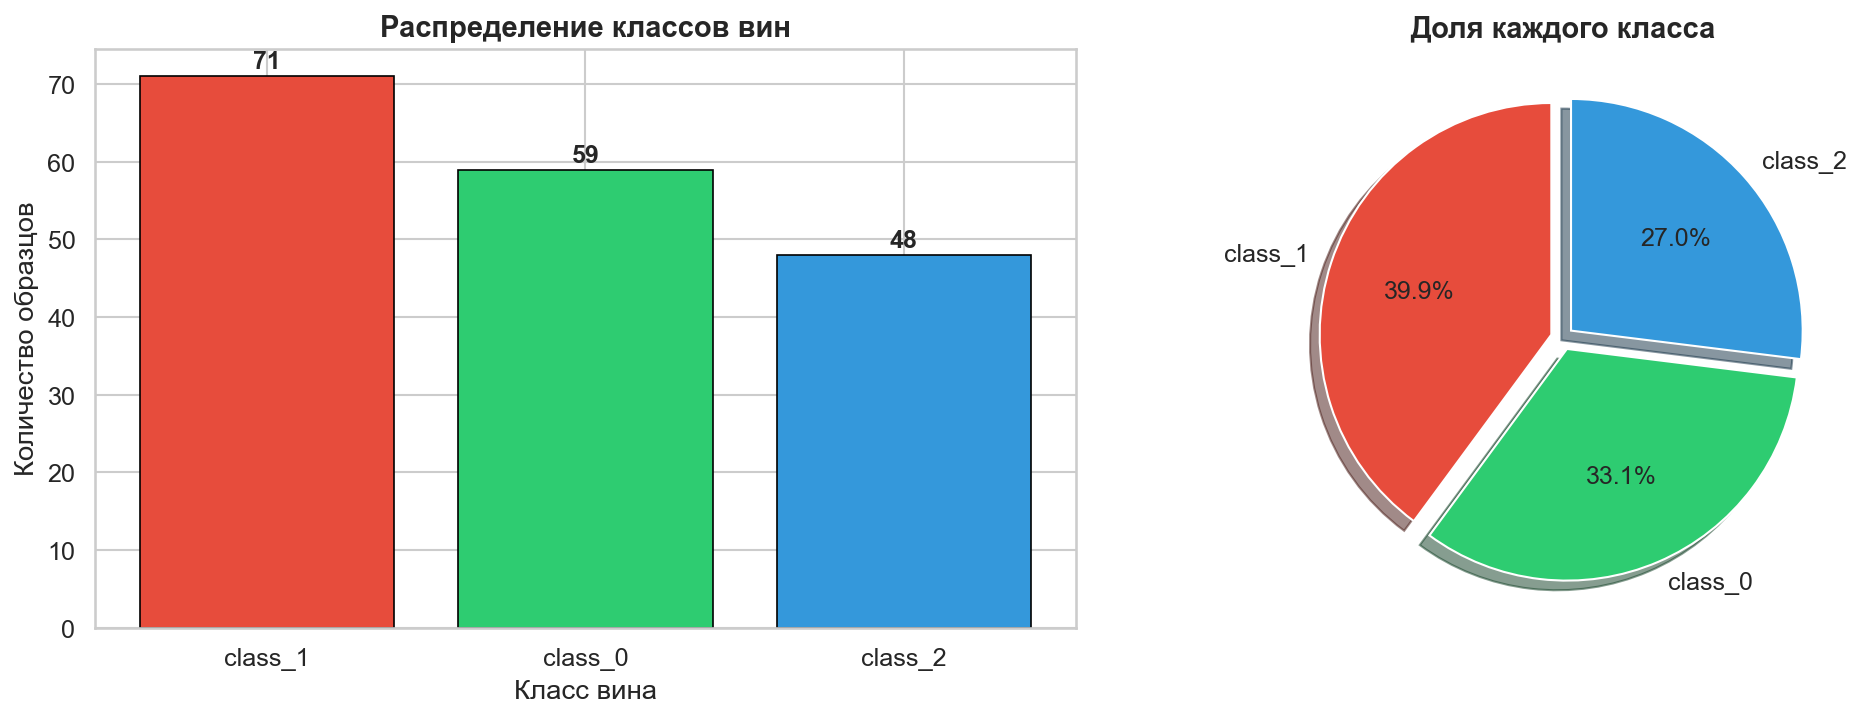
\includegraphics[width=0.85\textwidth]{fig_1.png}
    \newline
    \text Рисунок 1 --- Гистограммы распределения признаков по классам
    \newline
\end{figure}

\subsection*{Box plots для анализа распределений}
\begin{lstlisting}
# Box plots
fig, axes = plt.subplots(4, 4, figsize=(18, 14))
axes = axes.flatten()

for i, col in enumerate(wine.feature_names):
    ax = axes[i]
    sns.boxplot(data=df, x='target_name', y=col, ax=ax, palette=colors)
    ax.set_title(col, fontweight='bold')
    ax.set_ylabel('Значение')

plt.tight_layout()
plt.savefig('boxplots.png', dpi=150, bbox_inches='tight')
plt.show()
\end{lstlisting}

\begin{figure}[h!]
    \centering
    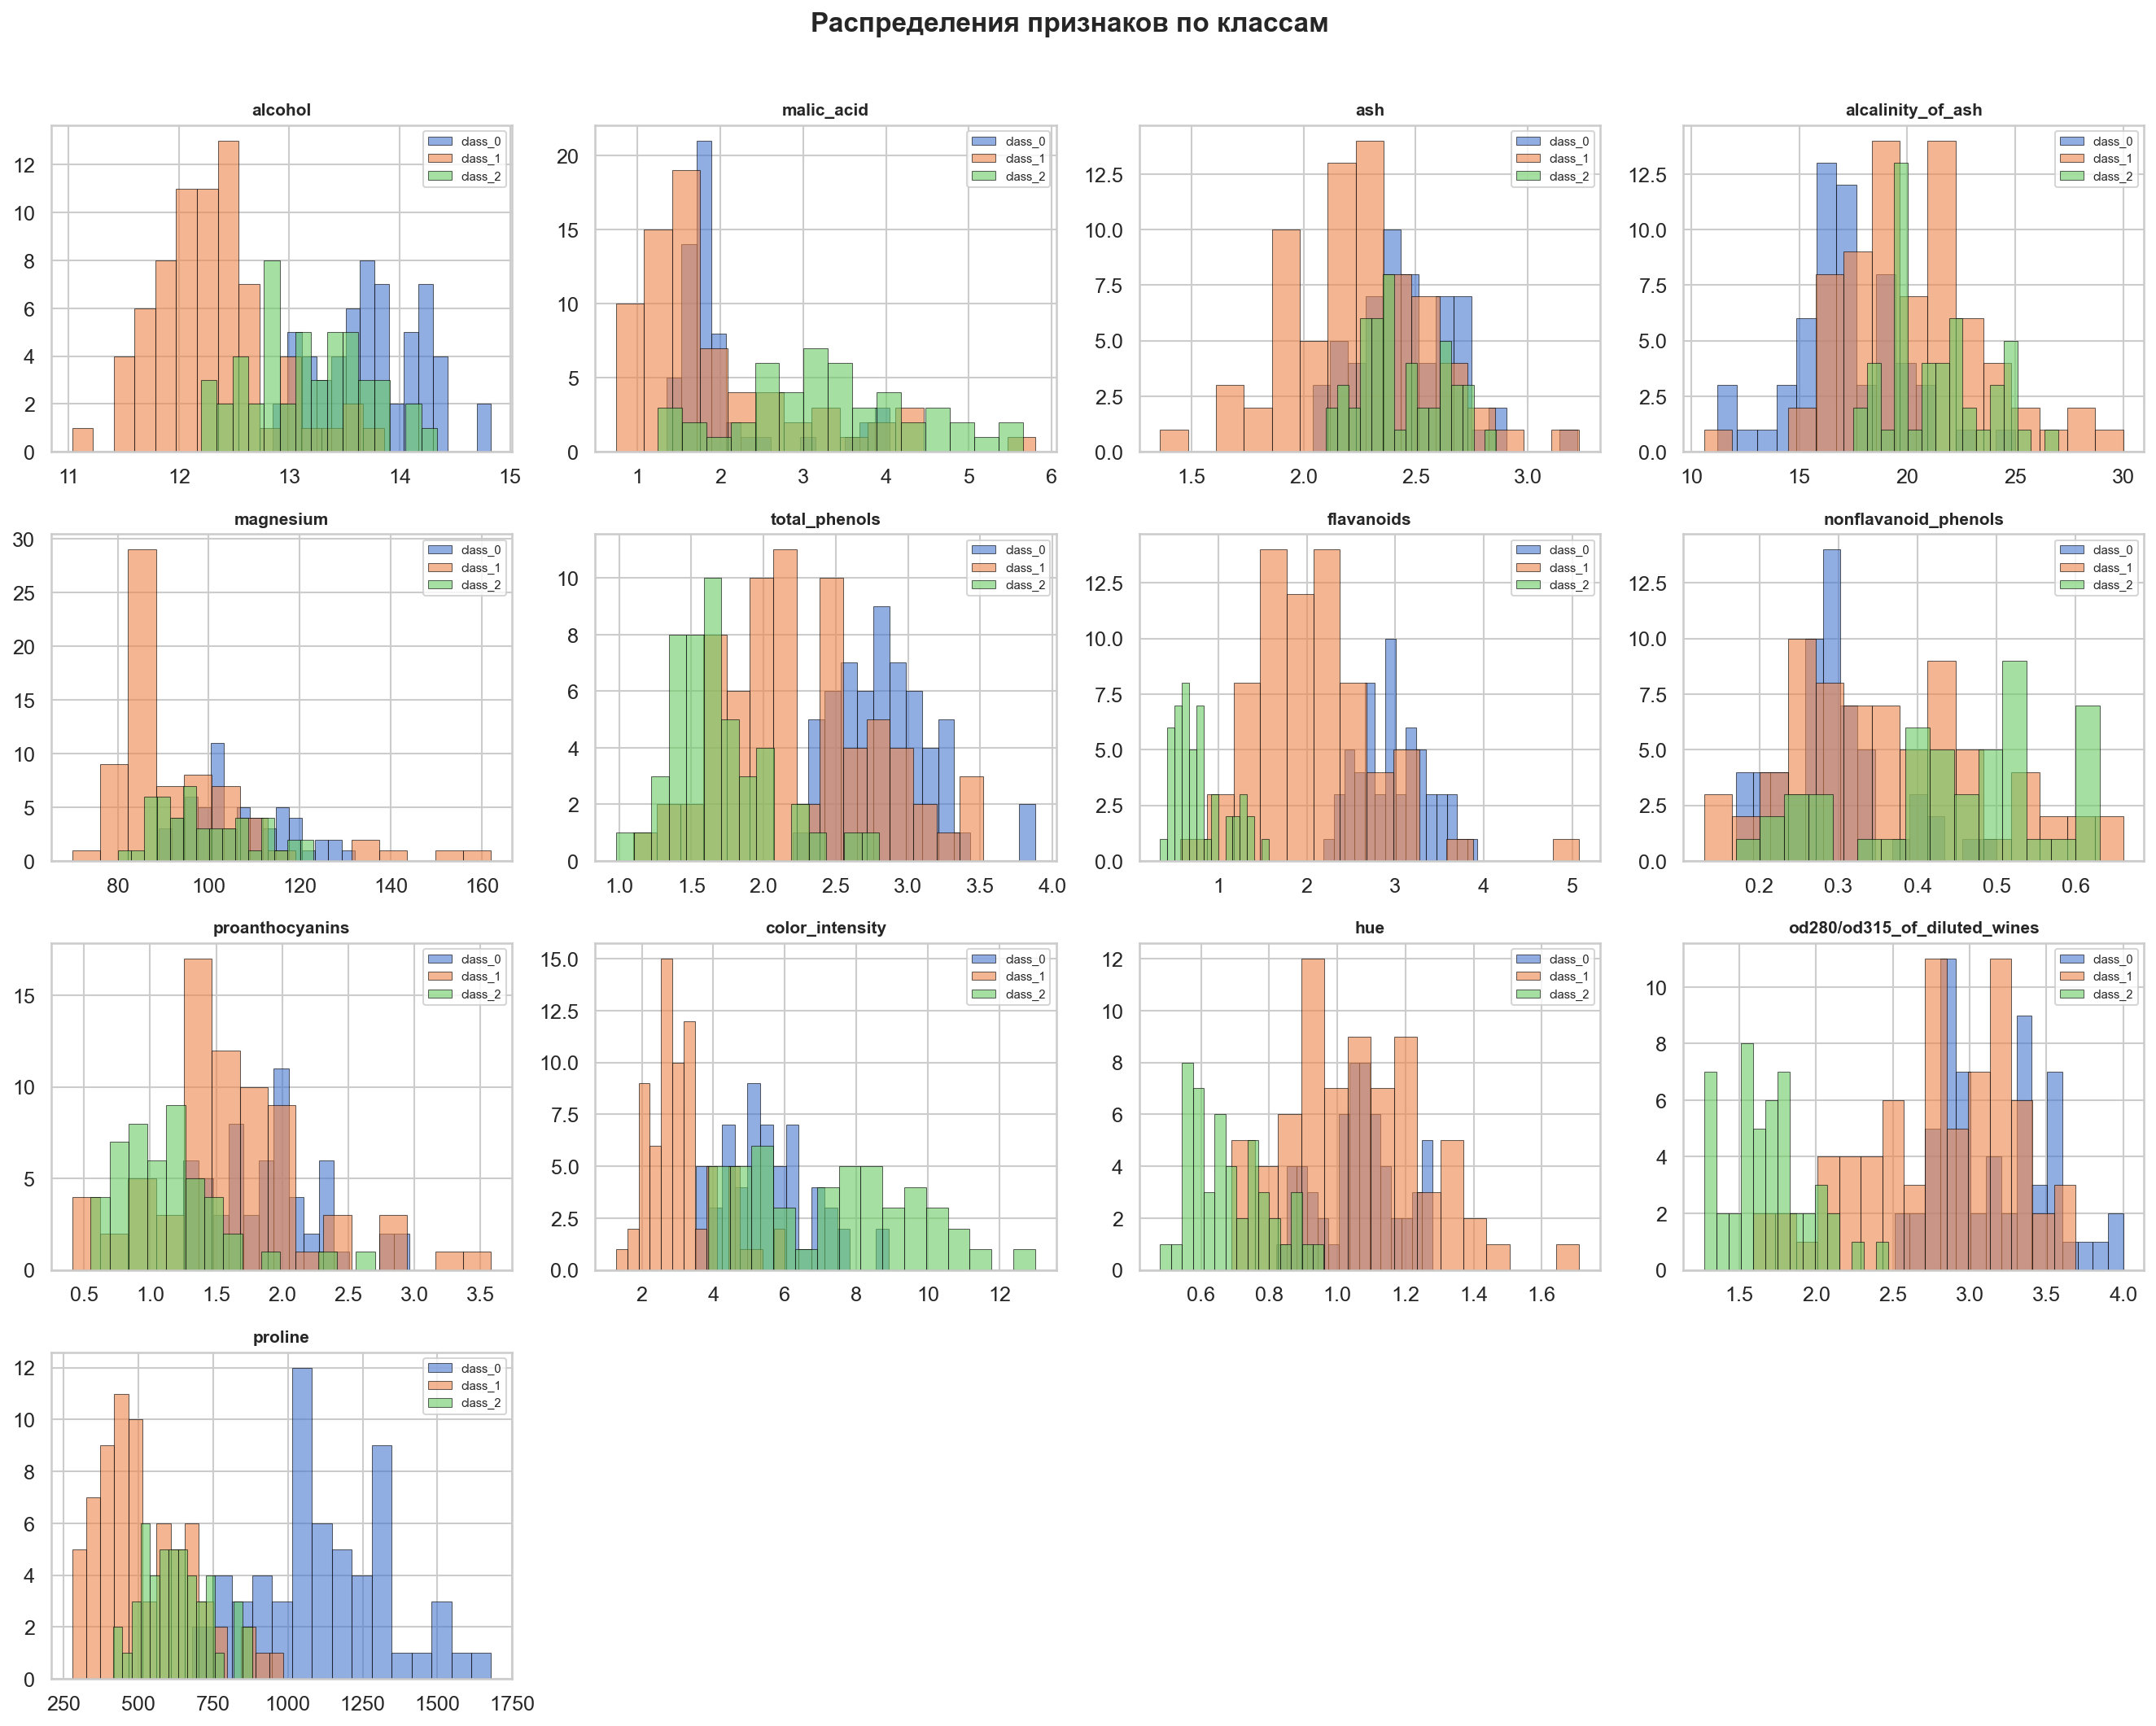
\includegraphics[width=0.85\textwidth]{fig_2.png}
    \newline
    \text Рисунок 2 --- Box plots для анализа распределений признаков по классам
    \newline
\end{figure}

\section*{Анализ корреляции признаков}

\subsection*{Корреляционная матрица}
\begin{lstlisting}
# Вычисление корреляции
corr_matrix = df[wine.feature_names].corr()

# Heatmap с корреляциями
fig, ax = plt.subplots(figsize=(14, 10))
mask = np.triu(np.ones_like(corr_matrix, dtype=bool))

sns.heatmap(corr_matrix, mask=mask, annot=True, fmt='.2f', 
            cmap='coolwarm', center=0, ax=ax, square=True)
ax.set_title('Корреляционная матрица признаков Wine', fontweight='bold', fontsize=14)

plt.tight_layout()
plt.savefig('correlation_matrix.png', dpi=150, bbox_inches='tight')
plt.show()

# Топ корреляций с целевой переменной
target_corr = df[wine.feature_names].corrwith(df['target']).sort_values(ascending=False)
print("\nТоп признаков по корреляции с целевой переменной:")
print(target_corr.head(5))
\end{lstlisting}

\begin{figure}[h!]
    \centering
    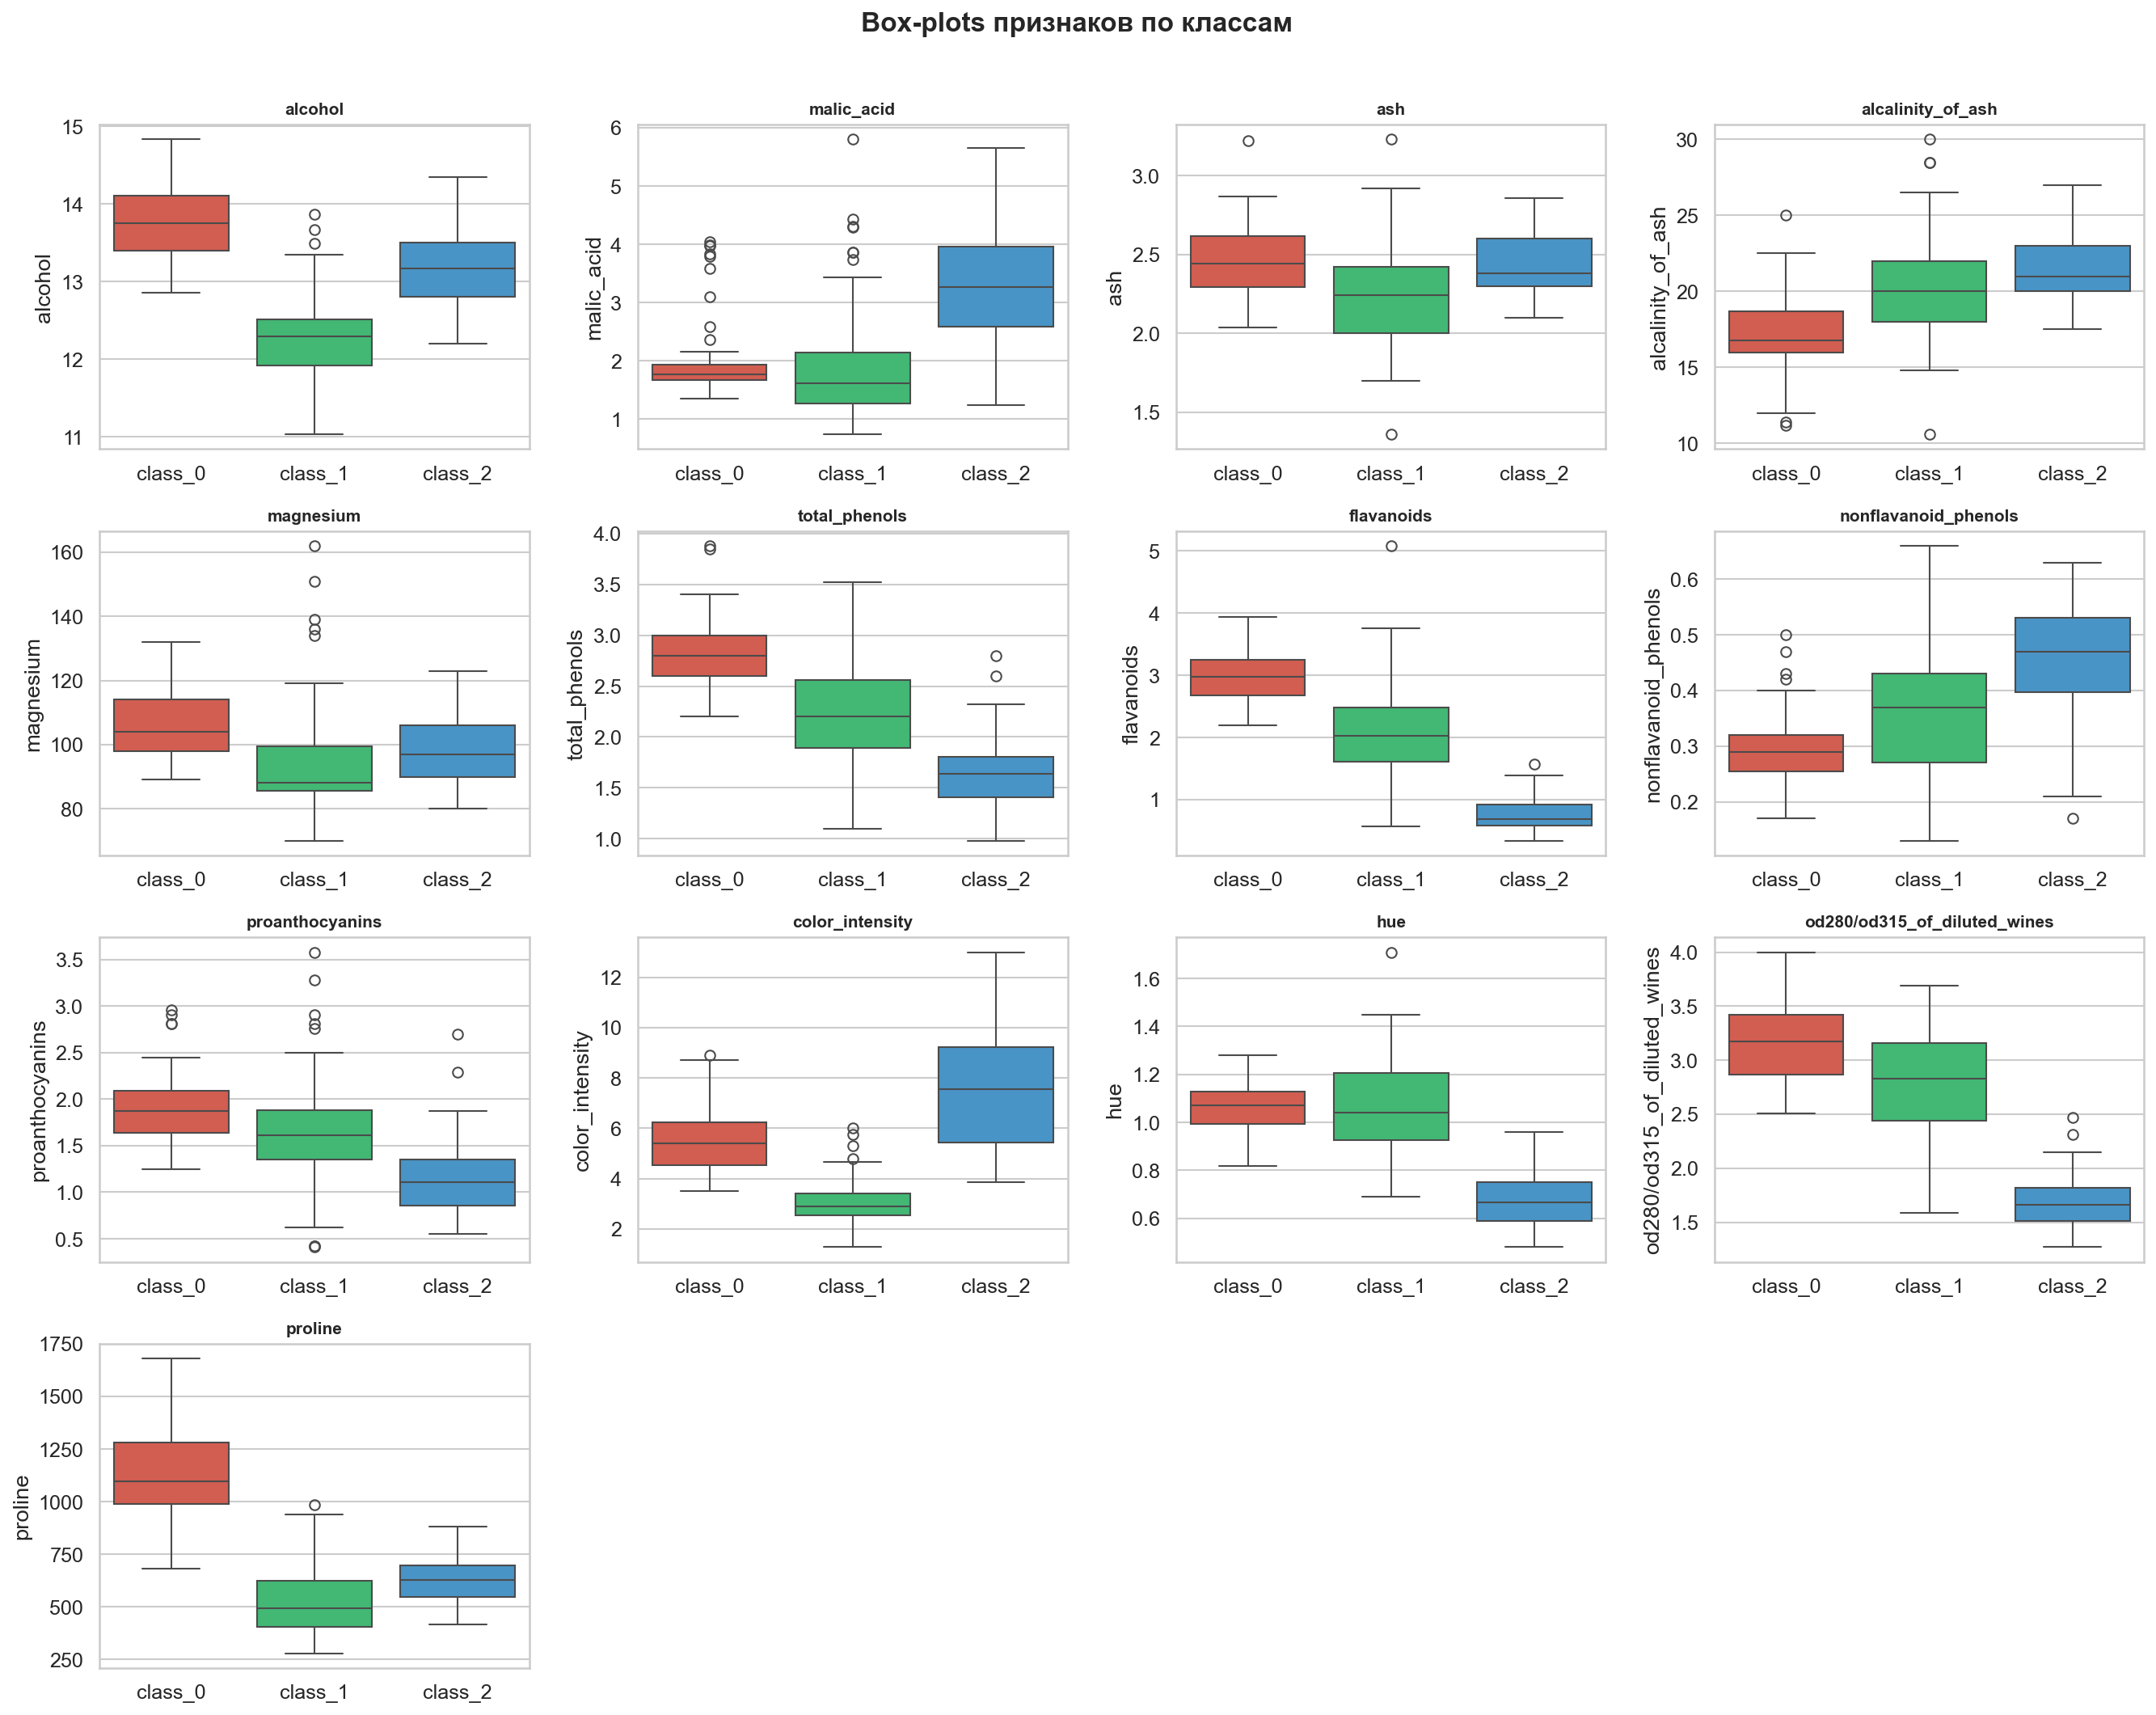
\includegraphics[width=0.85\textwidth]{fig_3.png}
    \newline
    \text Рисунок 3 --- Корреляционная матрица признаков датасета Wine
    \newline
\end{figure}

\subsection*{Ключевые корреляции}
\begin{itemize}
    \item \textbf{alcohol} ↔ \textbf{color\_intensity}: r ≈ 0.55 (положительная)
    \item \textbf{alcohol} ↔ \textbf{proline}: r ≈ 0.64 (положительная)
    \item \textbf{flavanoids} ↔ \textbf{color\_intensity}: r ≈ 0.65 (положительная)
    \item \textbf{malic\_acid} ↔ \textbf{alcohol}: r ≈ -0.32 (отрицательная)
\end{itemize}

\subsection*{Pairplot для избранных признаков}
\begin{lstlisting}
# Pairplot 
selected = ['alcohol', 'flavanoids', 'color_intensity', 'proline', 'target_name']
g = sns.pairplot(df[selected], hue='target_name', palette=colors,
                  diag_kind='kde', plot_kws={'alpha': 0.6, 's': 80})
g.fig.suptitle('Pairplot ключевых признаков Wine', y=1.001, fontsize=14)

plt.savefig('pairplot.png', dpi=150, bbox_inches='tight')
plt.show()
\end{lstlisting}

\begin{figure}[h!]
    \centering
    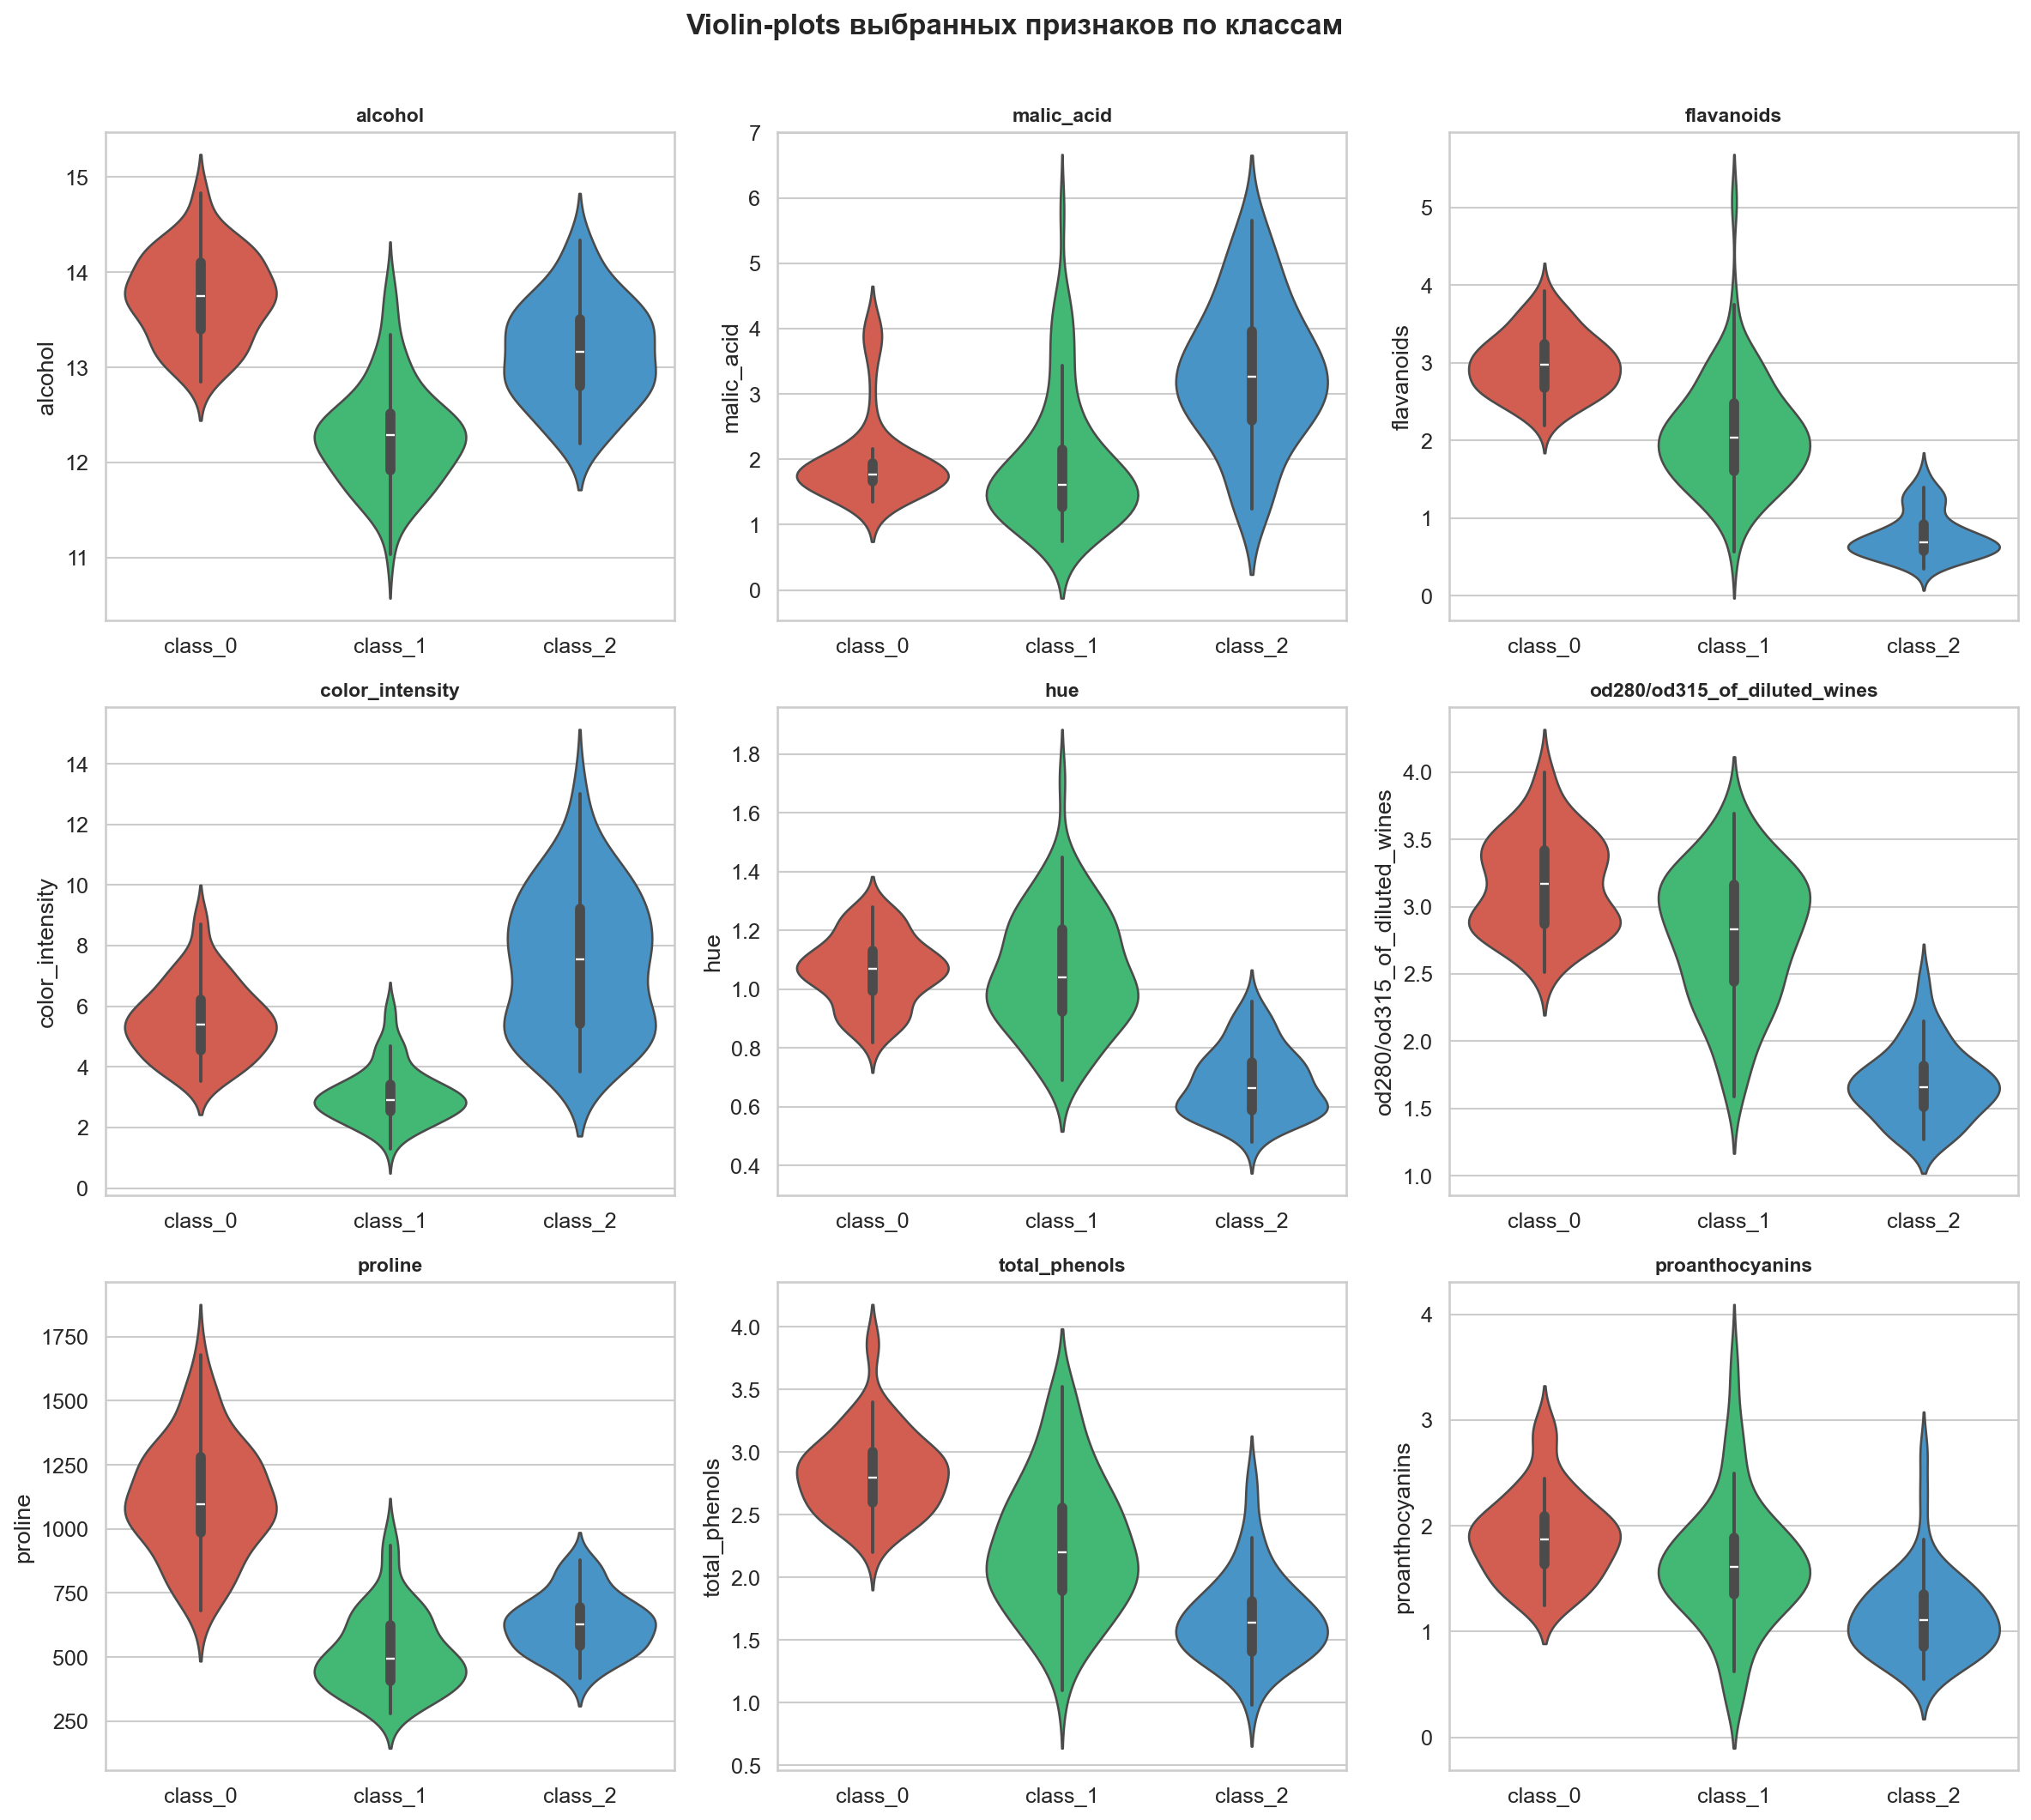
\includegraphics[width=0.85\textwidth]{fig_4.png}
    \newline
    \text Рисунок 4 --- Pairplot для ключевых признаков с разделением по классам
    \newline
\end{figure}

\subsection*{Дополнительные анализы}
\begin{lstlisting}
# Скрипл-плот распределения признаков
fig, axes = plt.subplots(2, 3, figsize=(15, 10))
# Visualize additional features...
plt.savefig('violin_plots.png', dpi=150, bbox_inches='tight')
plt.show()

# Скаттер-плоты пар признаков
fig, axes = plt.subplots(2, 2, figsize=(12, 10))
# Scatter plots for feature pairs...
plt.savefig('scatter_pairs.png', dpi=150, bbox_inches='tight')
plt.show()
\end{lstlisting}

\begin{figure}[h!]
    \centering
    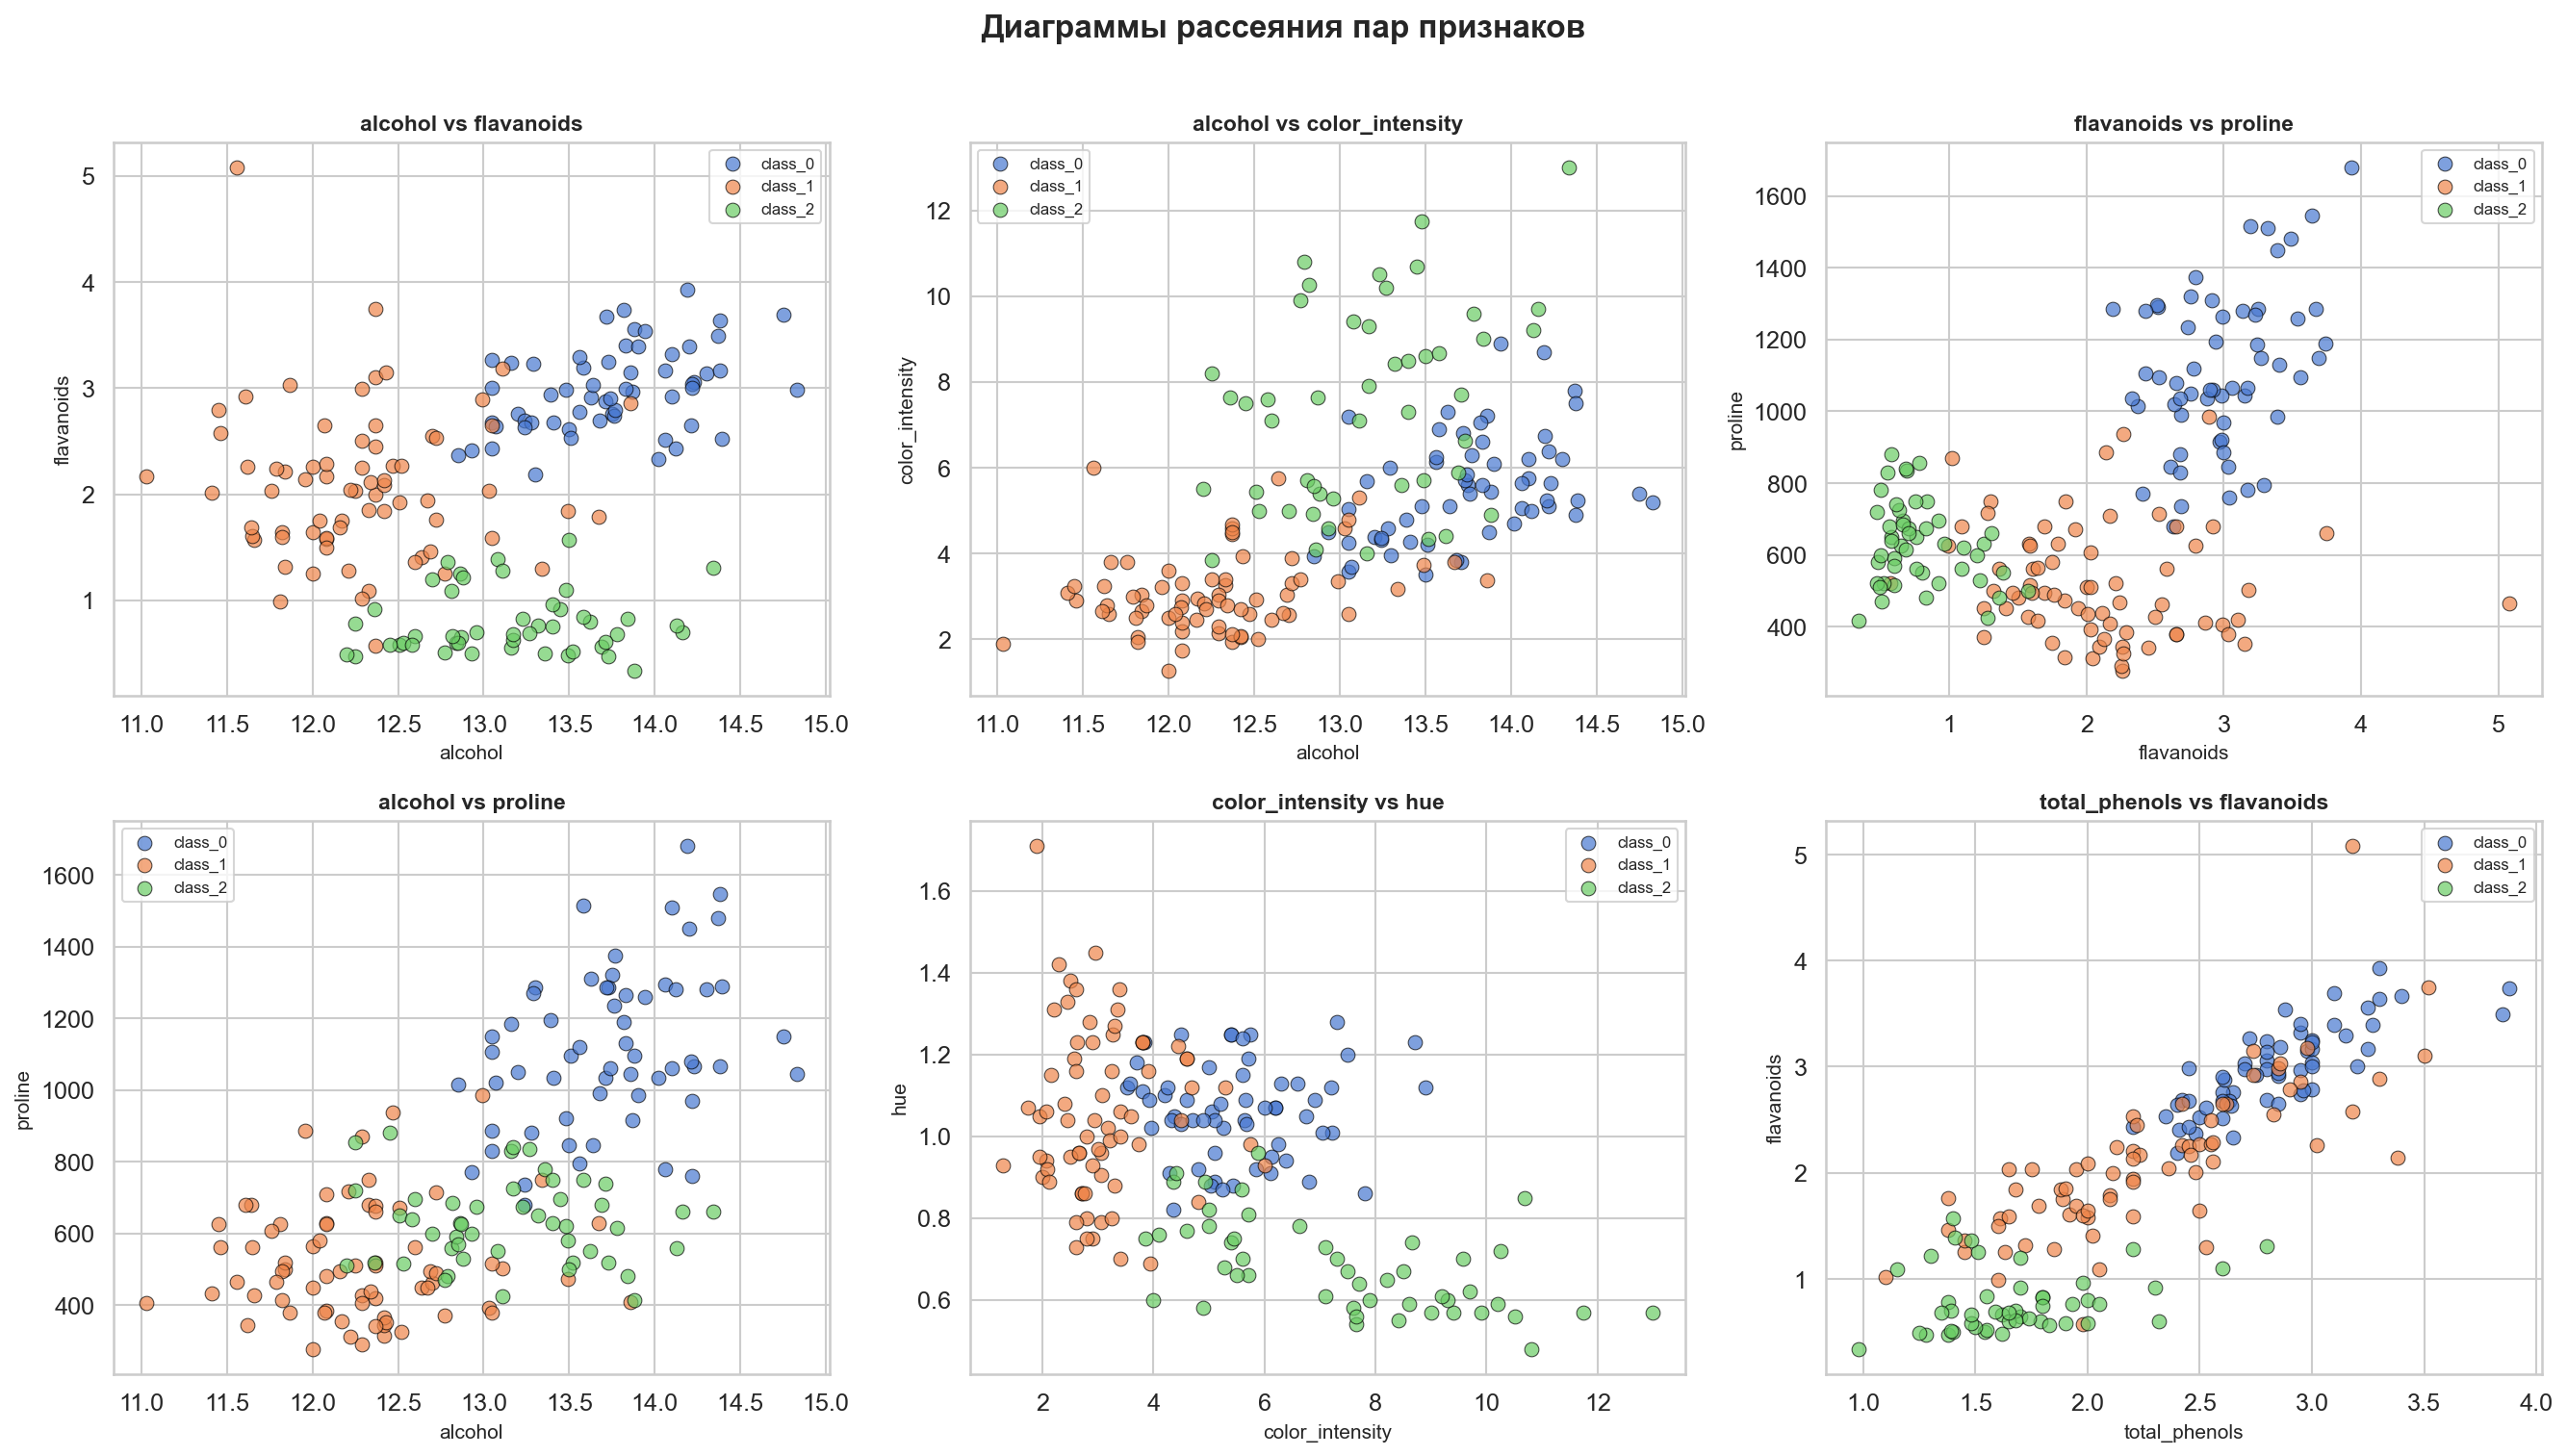
\includegraphics[width=0.85\textwidth]{fig_5.png}
    \newline
    \text Рисунок 5 --- Violin plots для отобранных признаков по классам
    \newline
\end{figure}

\begin{figure}[h!]
    \centering
    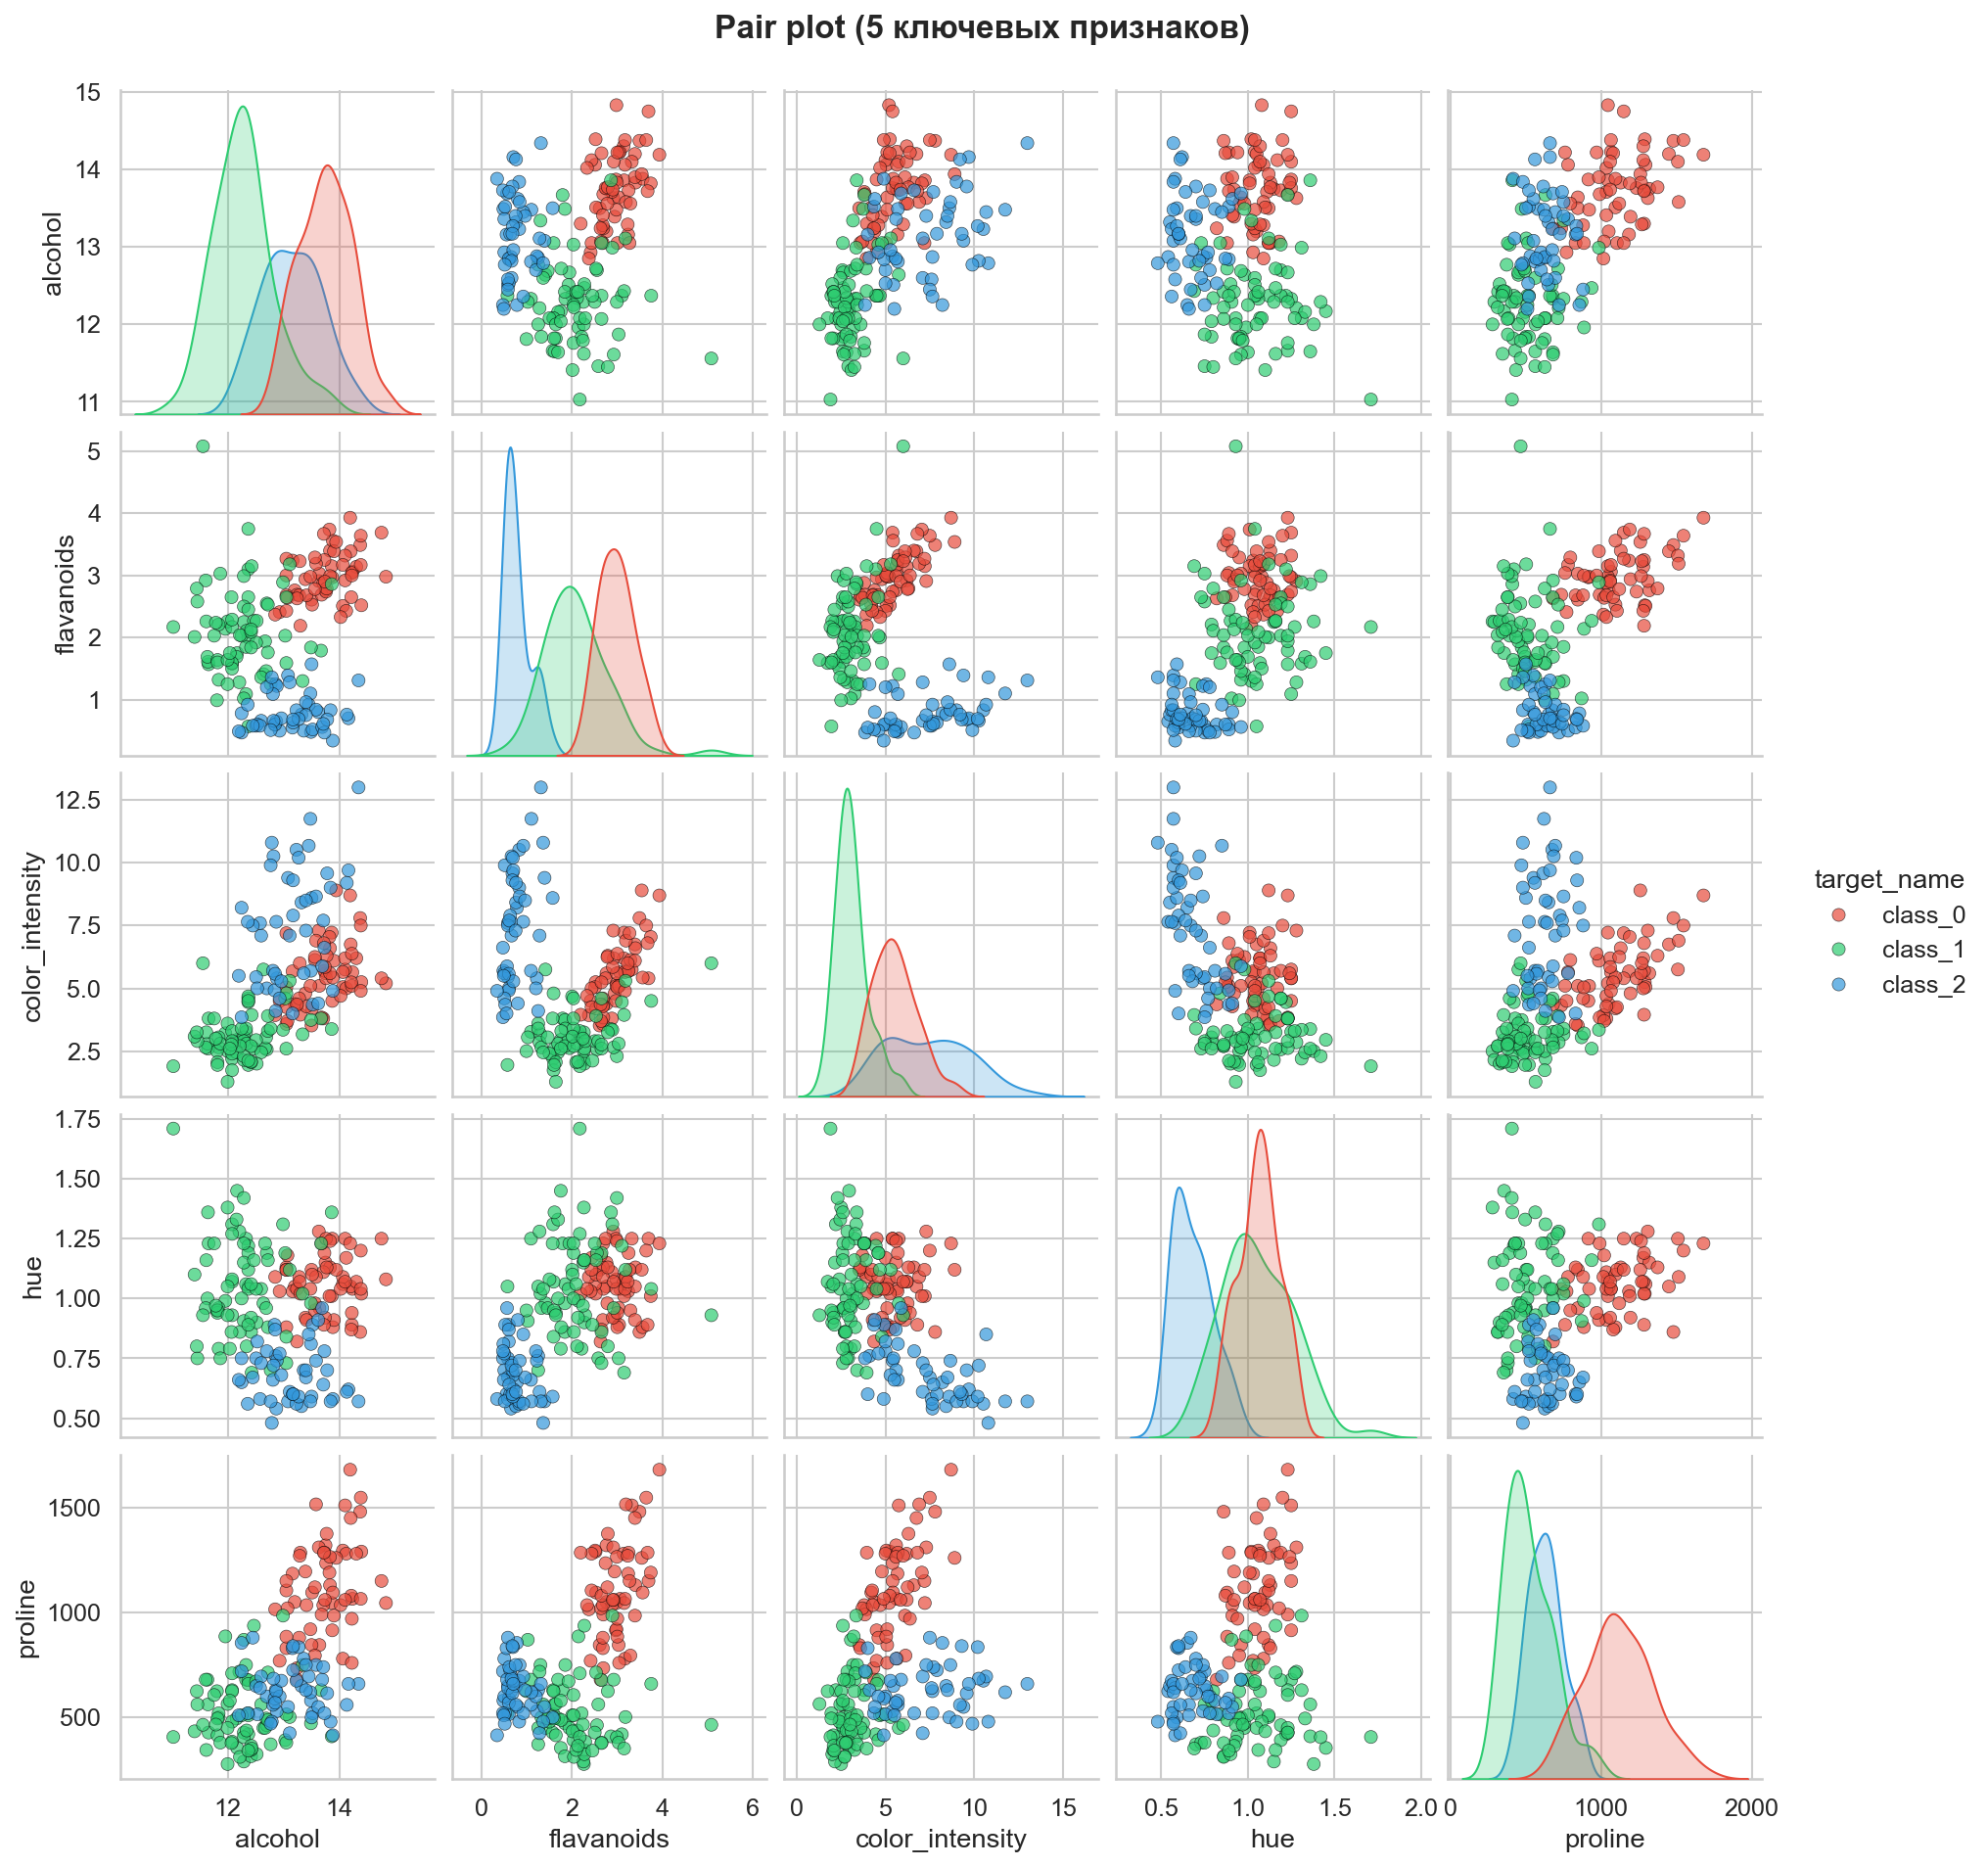
\includegraphics[width=0.85\textwidth]{fig_6.png}
    \newline
    \text Рисунок 6 --- Скаттер-плоты пар признаков с разделением по классам
    \newline
\end{figure}

\begin{figure}[h!]
    \centering
    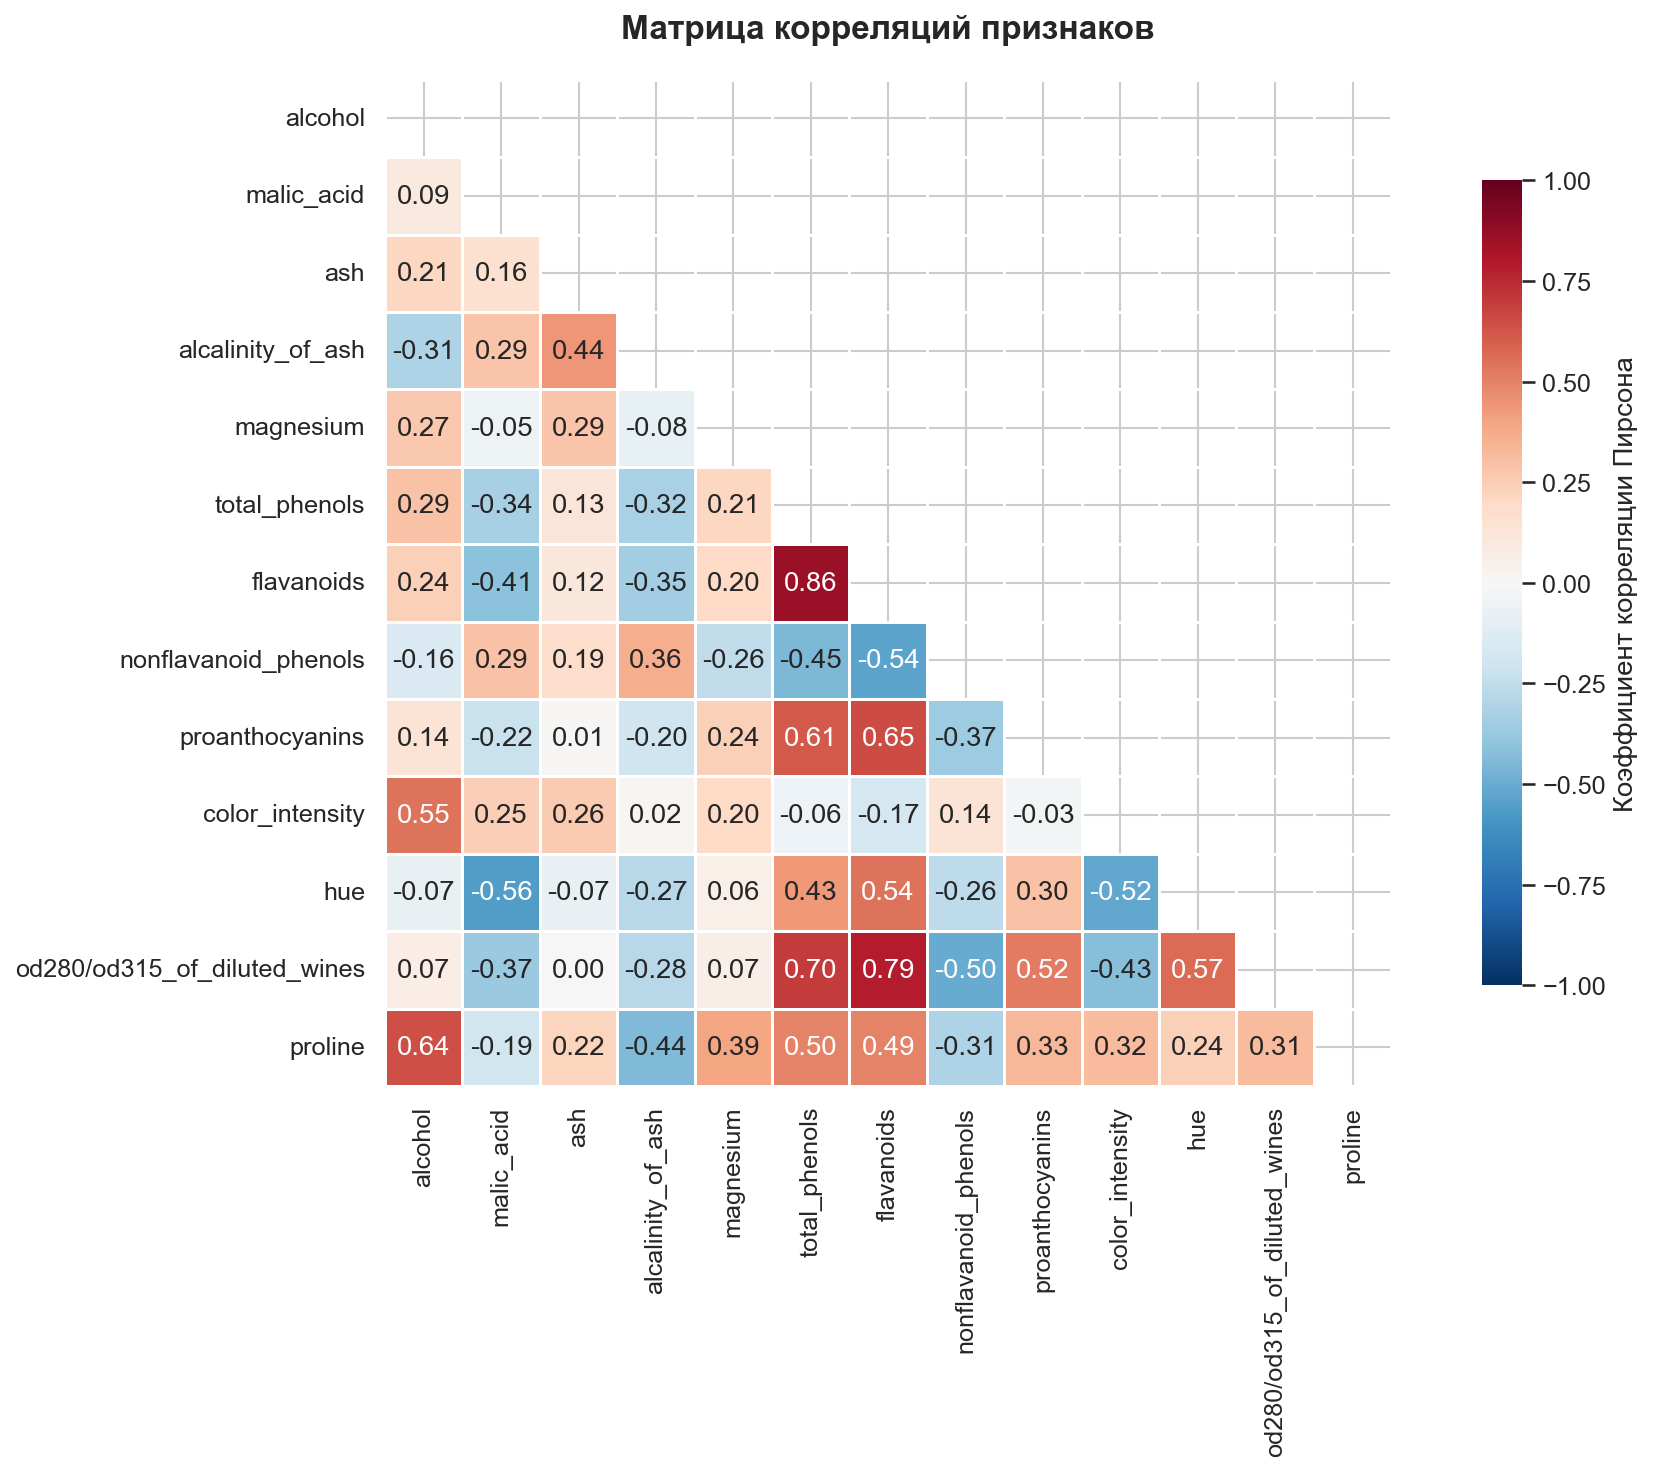
\includegraphics[width=0.85\textwidth]{fig_7.png}
    \newline
    \text Рисунок 7 --- Корреляция признаков с целевой переменной
    \newline
\end{figure}

\section*{Выводы}

\begin{enumerate}
    \item Датасет Wine хорошо структурирован без пропусков и легко разделяется на классы.
    \item Признаки \textbf{alcohol}, \textbf{flavanoids} и \textbf{color\_intensity} показывают наилучшую разделяющую способность.
    \item Обнаружены сильные положительные корреляции между рядом признаков (alcohol-proline, flavanoids-color\_intensity).
    \item Классы визуально хорошо отделяются в многомерном пространстве признаков.
\end{enumerate}

\end{document}
